

\chapter{IO}
\label{sec:IO}

This chapter introduces the mechanisms provided in the toolkit for reading and
writing images to files. Insight does not enforce any particular file format,
instead, it provides a structure to facilitate the future addition of file
formats without having to modify existing code. 



\section{Pluggable Factories}
\label{sec:ImageIOPluggableFactories}

\begin{figure}
\center
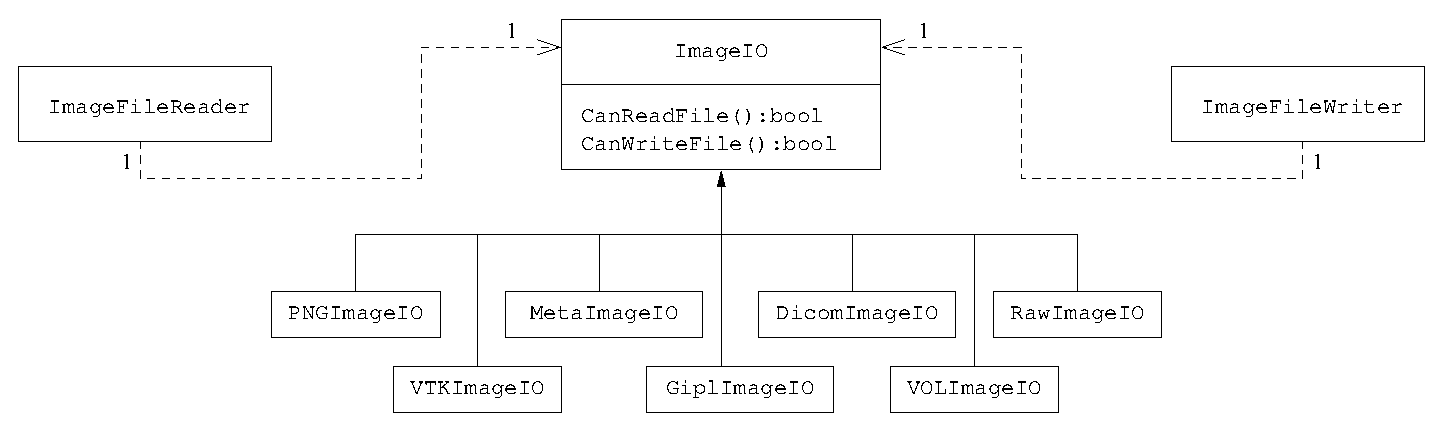
\includegraphics[width=12cm]{ImageIOCollaborationDiagram.eps}
\caption{Collaboration diagram of the ImageIO classes.}
\label{fig:ImageIOCollaborationDiagram}
\end{figure}


The principle behind the input/output mechanism is known as
\emph{pluggable-factories}. The concept is illustrated in the UML diagram in
figure \ref{fig:ImageIOCollaborationDiagram}. From the user's point of view the
objects responsible for reading and writing files are the
\code{itk::ImageFileReader} and \code{itk::ImageFileWriter} classes. These two
classes, however, are not aware of the details involved in reading or writing
particular file formats like PNG or DICOM.  What they do, is to dispatch the
user's requests to a set of specific classes that are aware of the file formats
intricacies. These classes are the ImageIO classes. The delegation mechanism
allows to extend the number of supported file formats by just adding new classes
to the ImageIO hierarchy.

\begin{figure}
\center
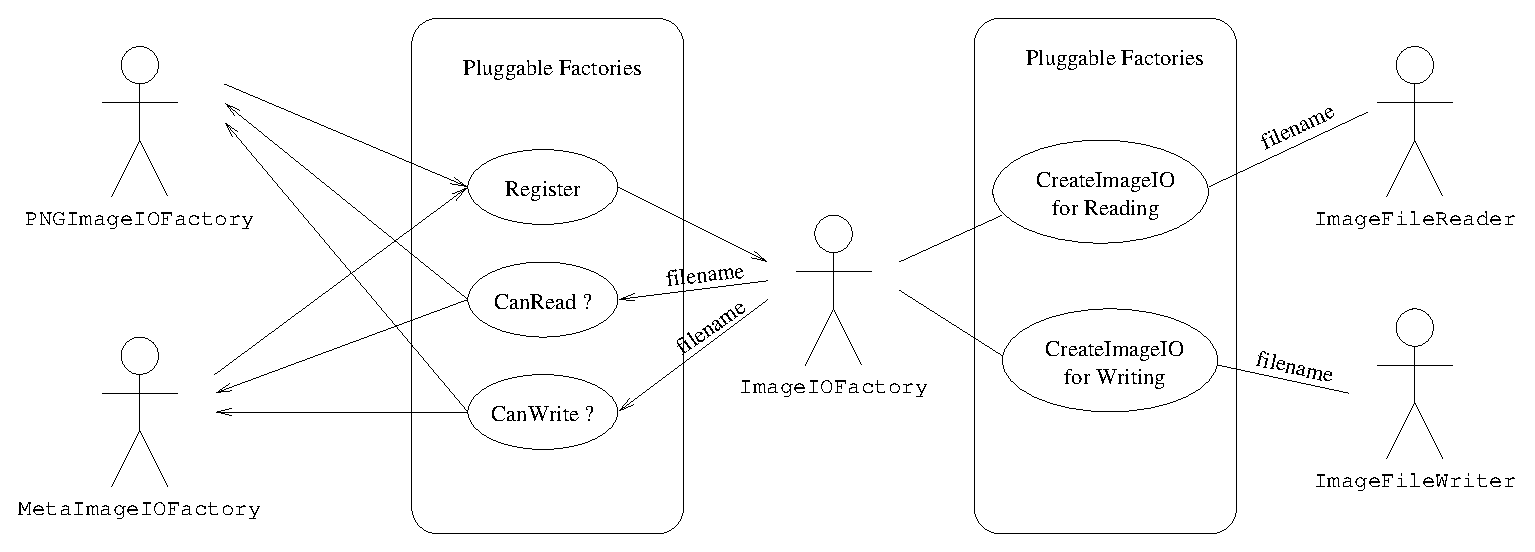
\includegraphics[width=13cm]{ImageIOFactoriesUseCases.eps}
\caption{Use cases of ImageIO factories}
\label{fig:ImageIOFactoriesUseCases}
\end{figure}


Each instance of \code{itk::ImageFileReader} and \code{itk::ImageFileWriter}
has a pointer to an ImageIO object. If this pointer is empty, it will be
impossible to read/write an image and any request for doing so will result in
an exception being thrown. When a request for reading or writing a file is
passed to any ImageFile object, it attempts to find an appropriate ImageIO
object capable of doing the job. This is done basically by passing the filename
to a centralized class, the \code{ImageIOFactory} and asking it if it knows of
any ImageIO class capable of reading/writing this file. This is illustrated by
the use cases on the right side of figure \ref{fig:ImageIOFactoriesUseCases}.

Each class derived from ImageIO should provide an associated factory class
capable of producing an instance of the ImageIO class. For example, for PNG
files, there is a PNGImageIO object that knows how to read this image files
and there is a PNGImageIOFactory class capable of constructing a PNGImageIO
object and returning its pointer. Each time a new file format is added, its
factory should be implemented as a derived class of the \code{ImageIOFactory}
class as illustrated in figure \ref{fig:ImageIOFactoriesClassDiagram}. 

\begin{figure}
\center
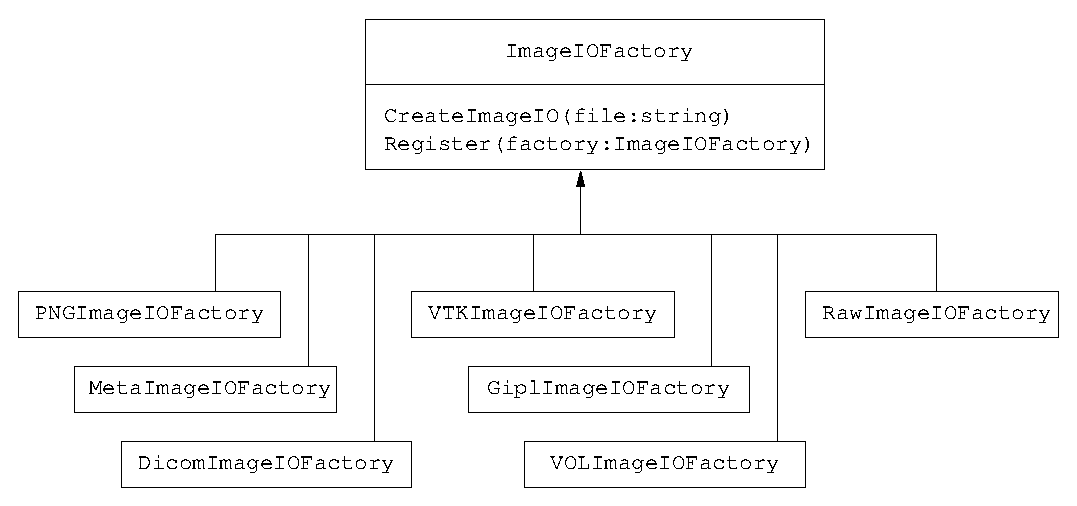
\includegraphics[width=10cm]{ImageIOFactoriesClassDiagram.eps}
\caption{Class diagram of ImageIO factories.}
\label{fig:ImageIOFactoriesClassDiagram}
\end{figure}

In order to read PNG files, a PNGImageIOFactory should be created and
registered with the central ImageIOFactory singleton\footnote{\emph{Singleton}
means that there is only one instance of this class in a particular
application} class as illustrated in the left side of figure
\ref{fig:ImageIOFactoriesUseCases}. When the ImageFileReader asks the
ImageIOFactory for an ImageIO capable of reading the file identified with
\emph{filename} the ImageIOFactory will iterate over the list of registered
factories and will ask each one of them is they know how to read the file. The
factory that responds afirmatively will be used to create the specific ImageIO
instance that will be returned to the \code{ImageFileReader}.

In most cases the whole mechanism will be transparent to the user who will only
interact with the \code{ImageFileReader} and \code{ImageFileWriter}. The following
sections introduce specific examples of commonly used IO tasks. 




